\section{Các diagram trong bài tập lớn}
\subsection{Class diagram tổng quát}
\begin{figure}[H]
\centering
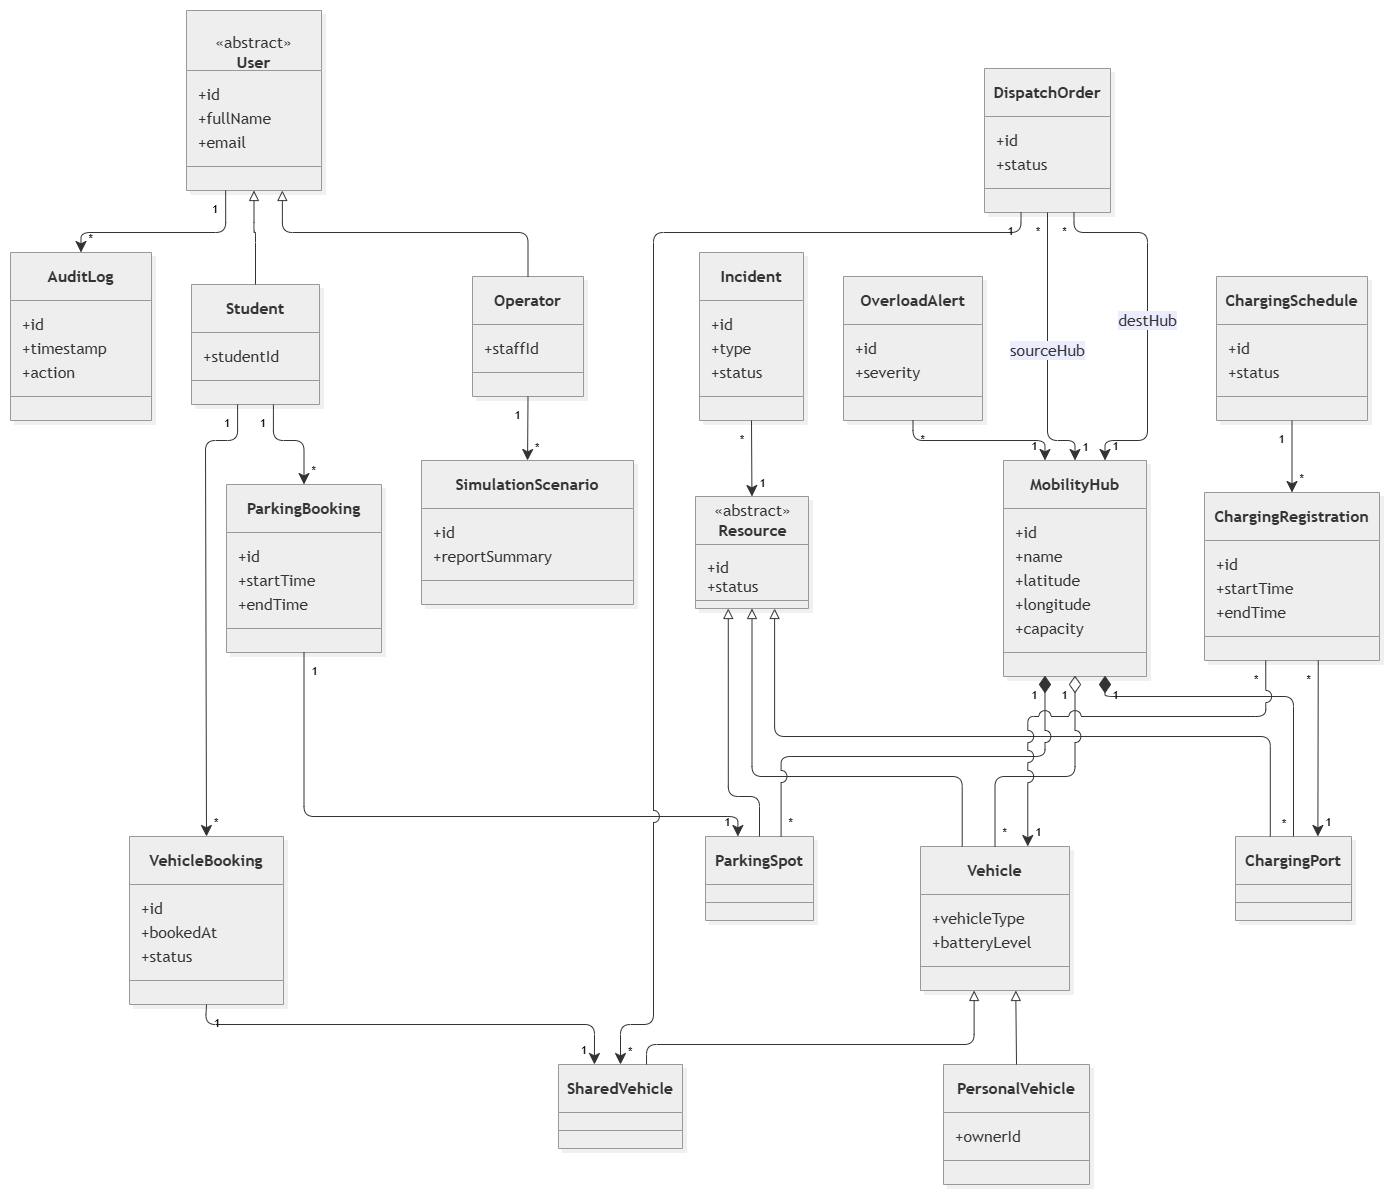
\includegraphics[width=\textwidth,height=0.82\textheight,keepaspectratio]{s3/class_diagram_submission3.drawio.png}
\end{figure}
\clearpage

\subsection{Deployment view}
\begin{figure}[H]
\centering
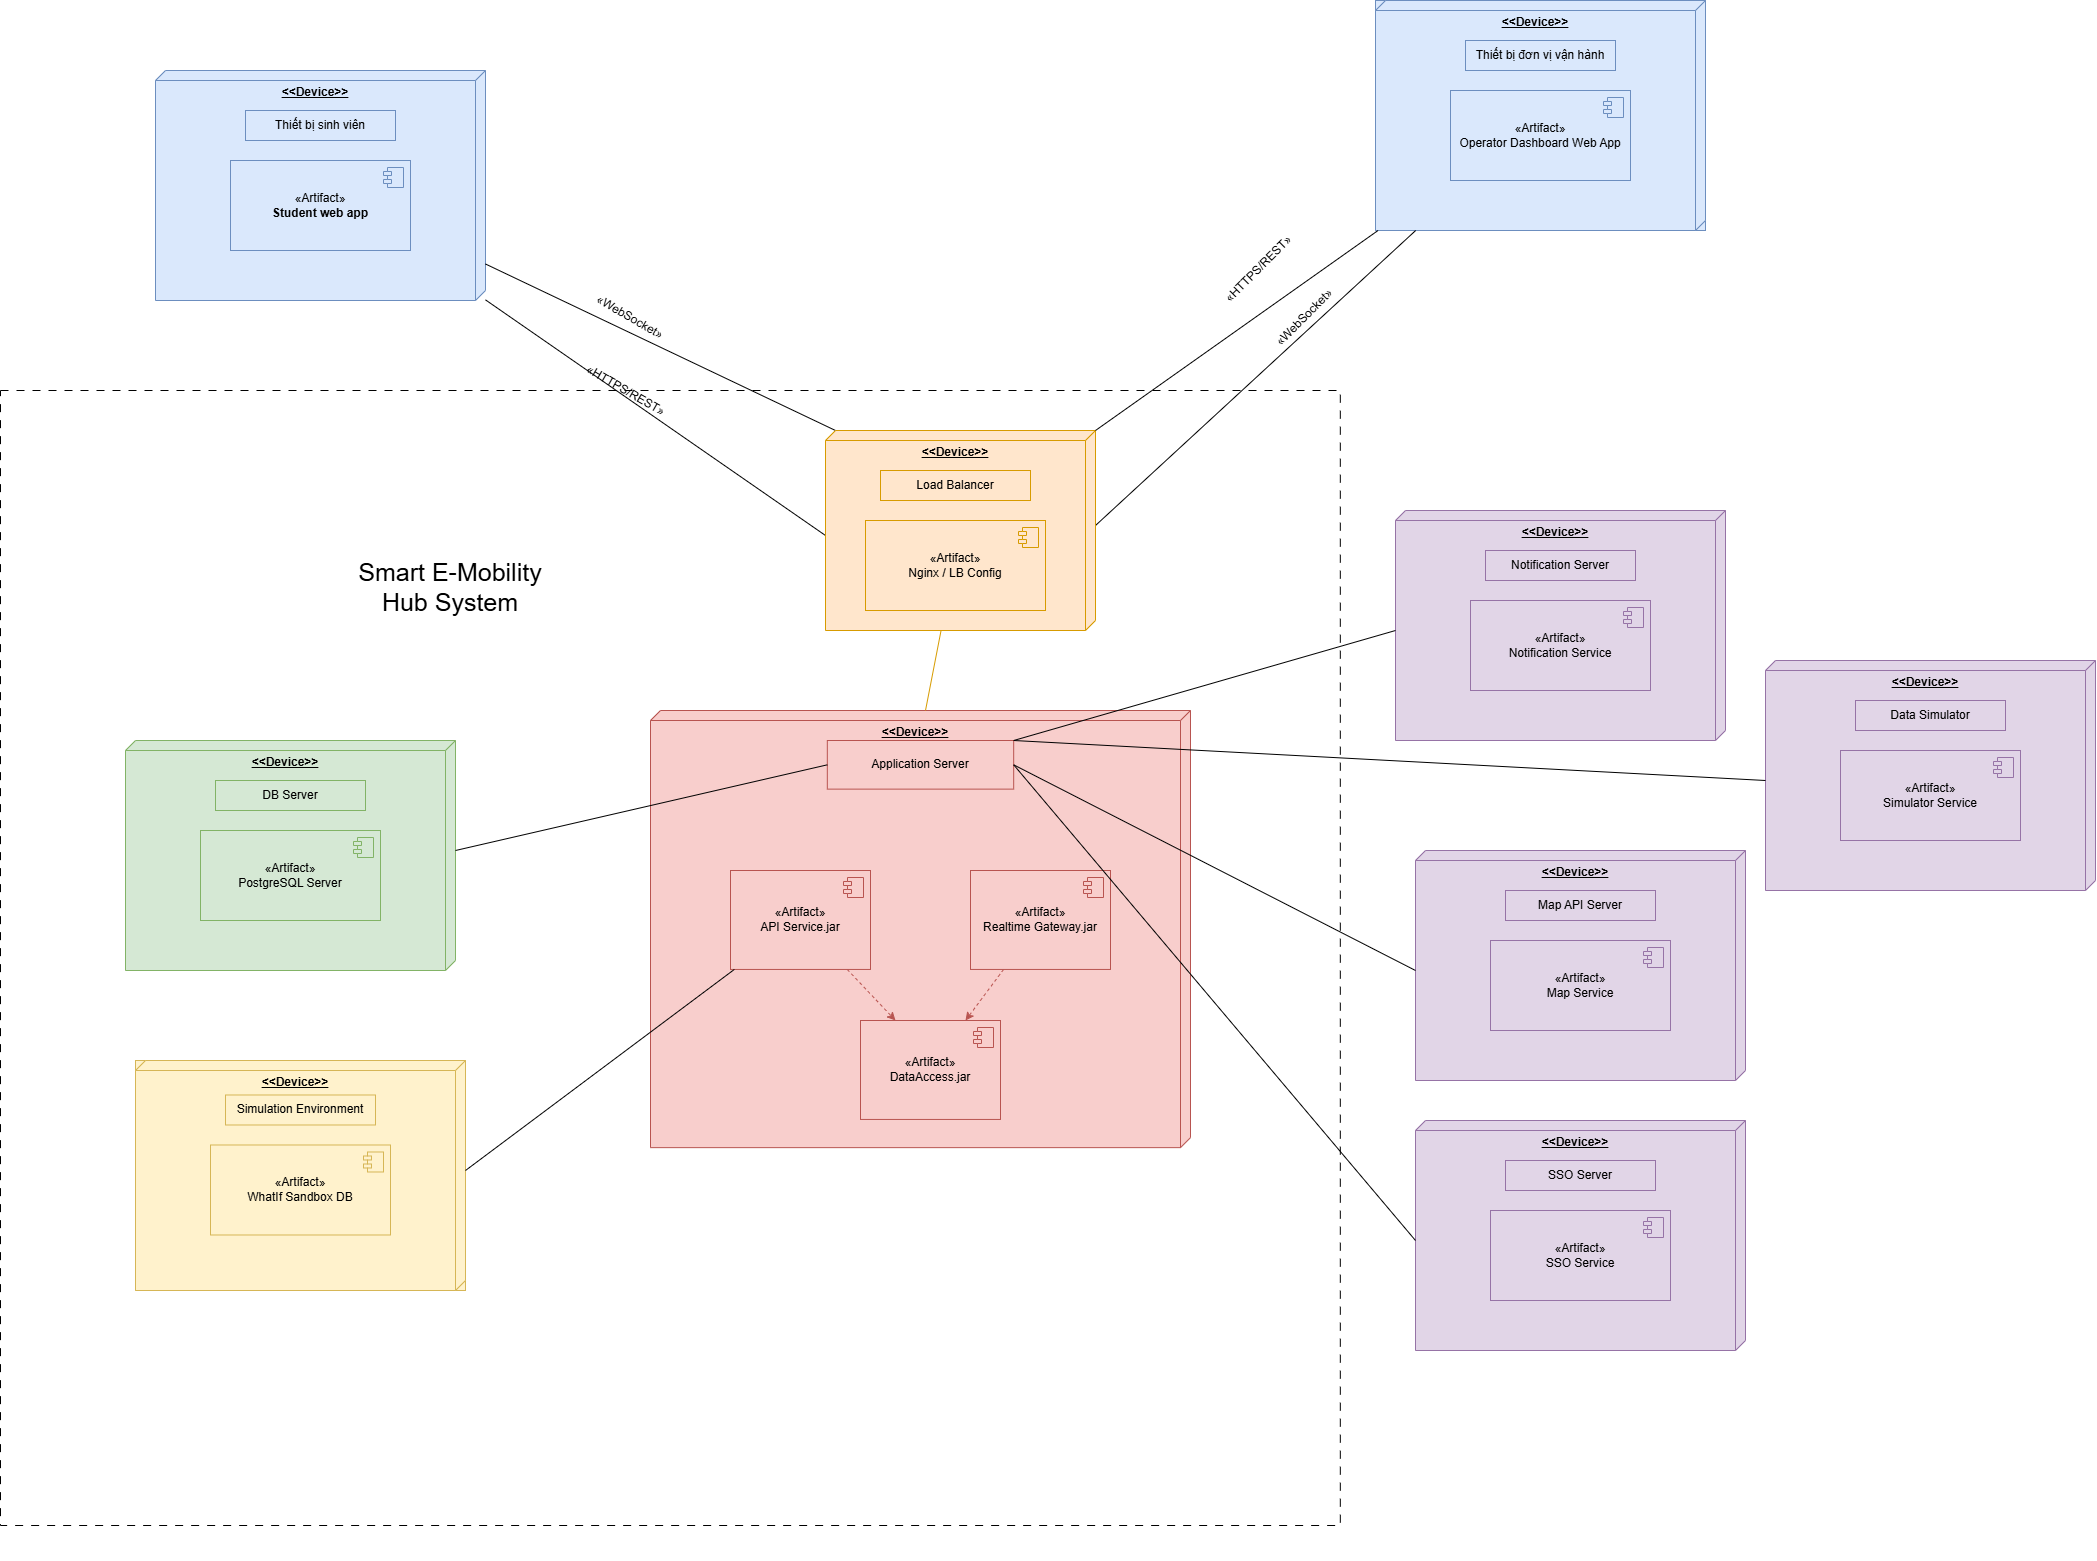
\includegraphics[width=\textwidth,height=0.82\textheight,keepaspectratio]{s3/deployment_view.drawio.png}
\end{figure}
\clearpage

\subsection{Implementation view}
\begin{figure}[H]
\centering
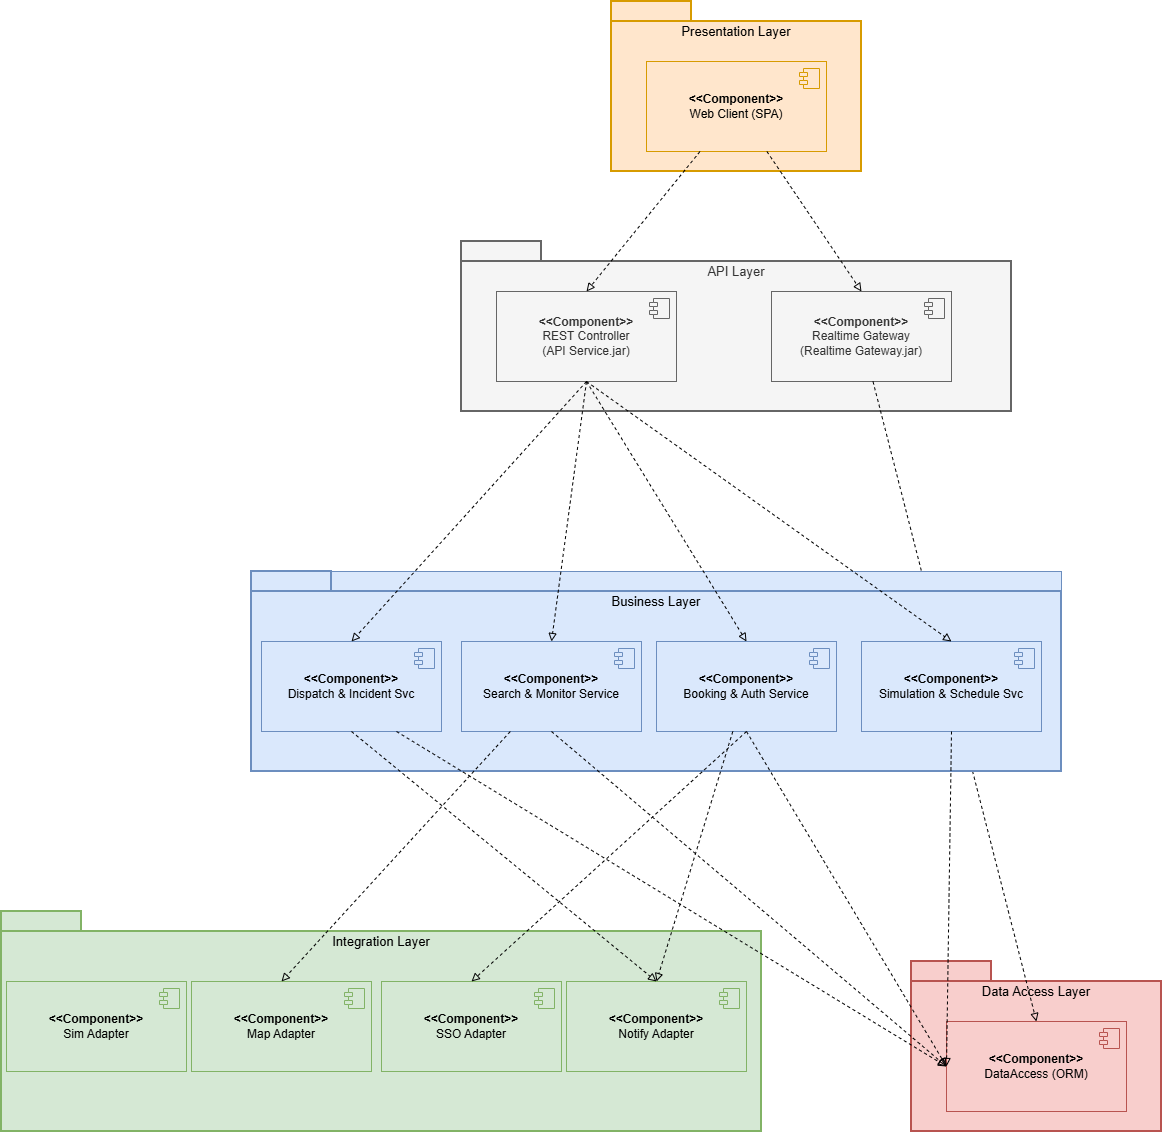
\includegraphics[width=\textwidth,height=0.82\textheight,keepaspectratio]{s3/implementation_view.drawio.png}
\end{figure}
\clearpage

\subsection{Class diagram UC1, UC2, UC8}
\begin{figure}[H]
\centering
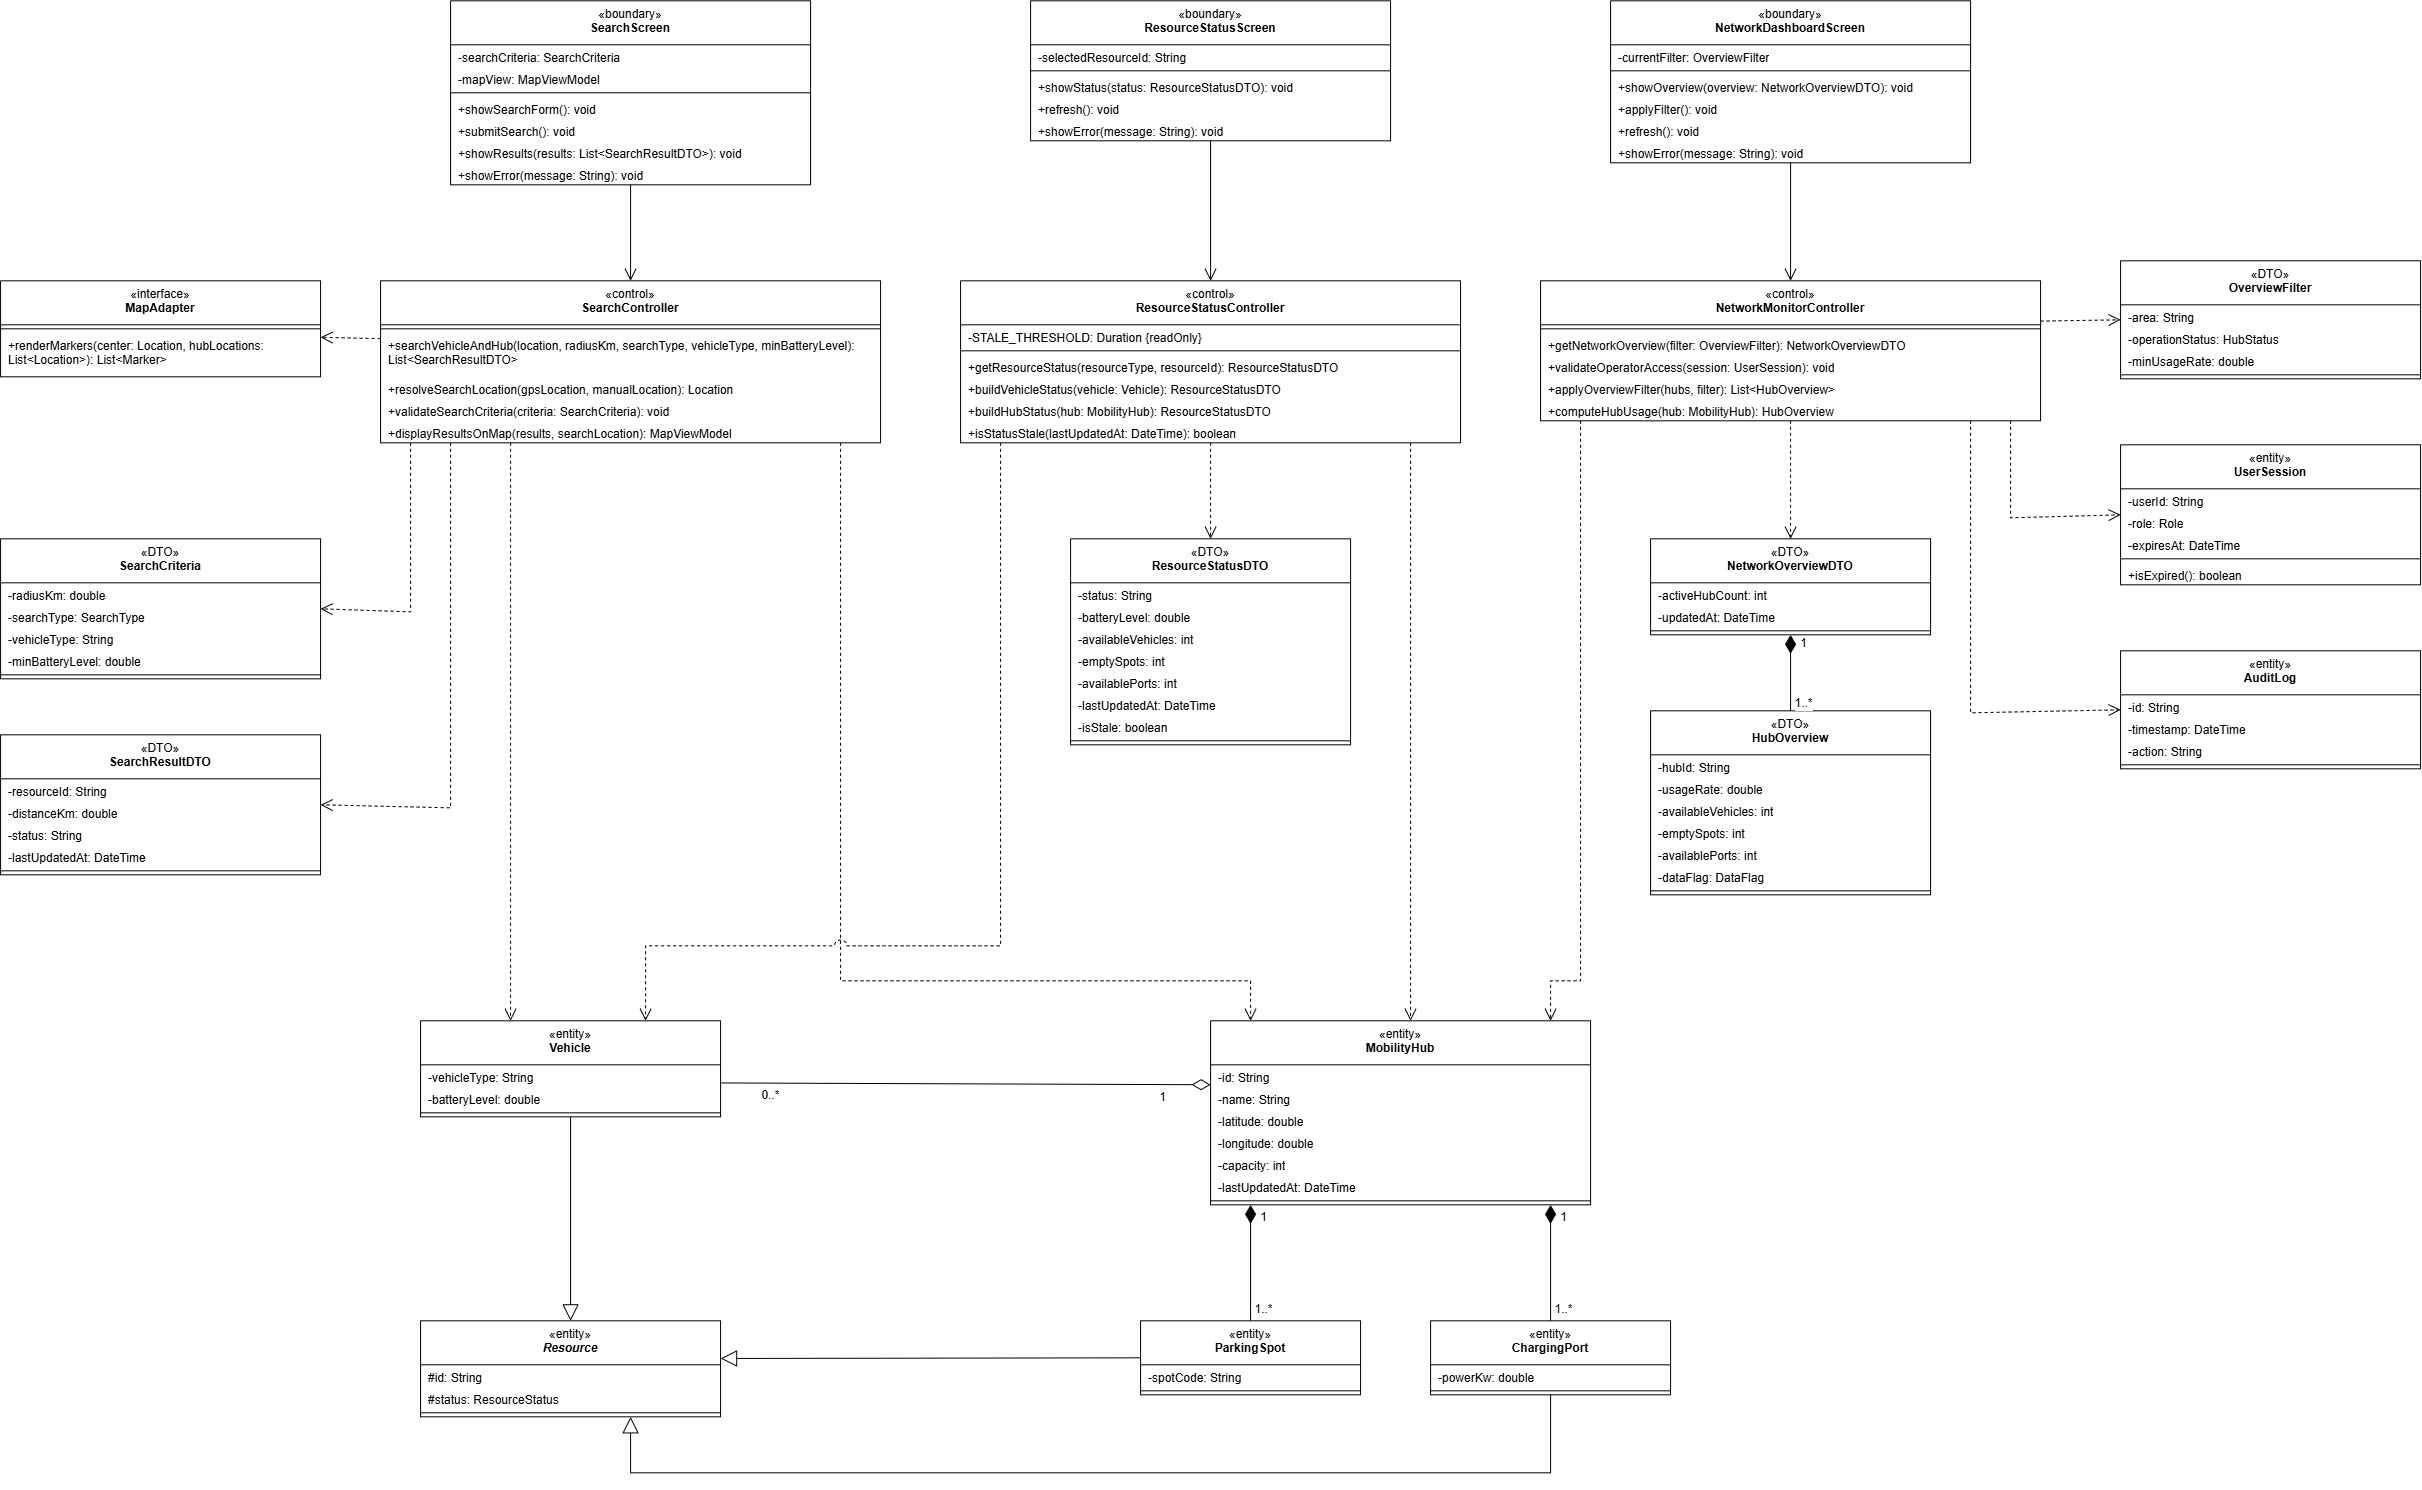
\includegraphics[width=\textwidth,height=0.82\textheight,keepaspectratio]{s3/ClassDiagram_UC1_UC2_UC8.png}
\end{figure}
\clearpage

\subsection{Class diagram UC3, UC4, UC5, UC17}
\begin{figure}[H]
\centering
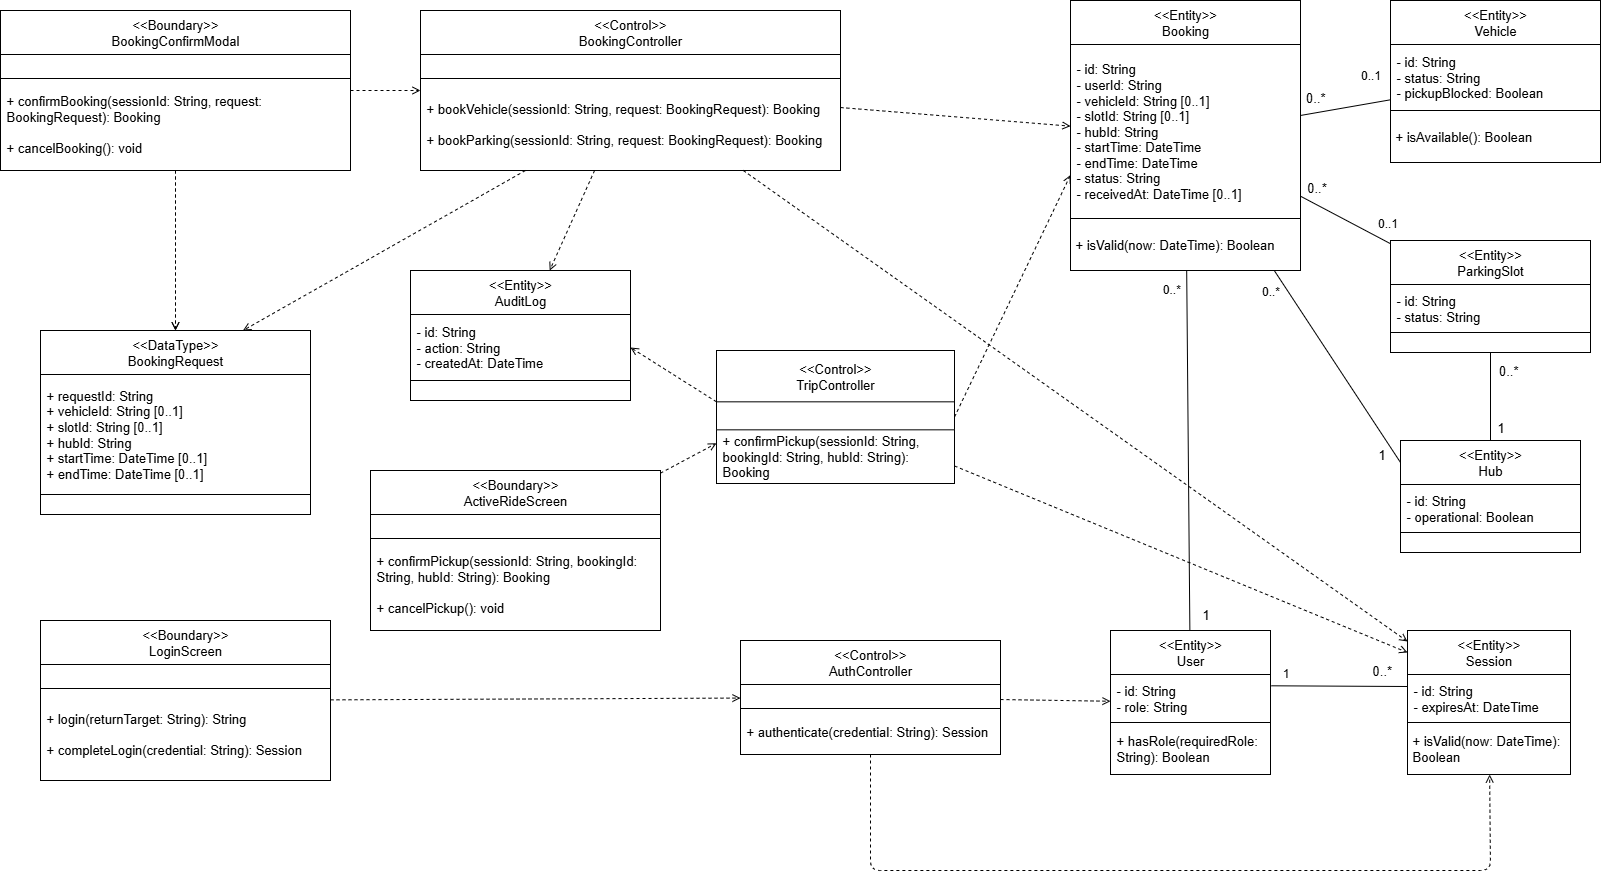
\includegraphics[width=\textwidth,height=0.82\textheight,keepaspectratio]{s3/Class_diagram_UC_3_4_5_17.png}
\end{figure}
\clearpage

\subsection{Class diagram UC6, UC7, UC9, UC10}
\begin{figure}[H]
\centering
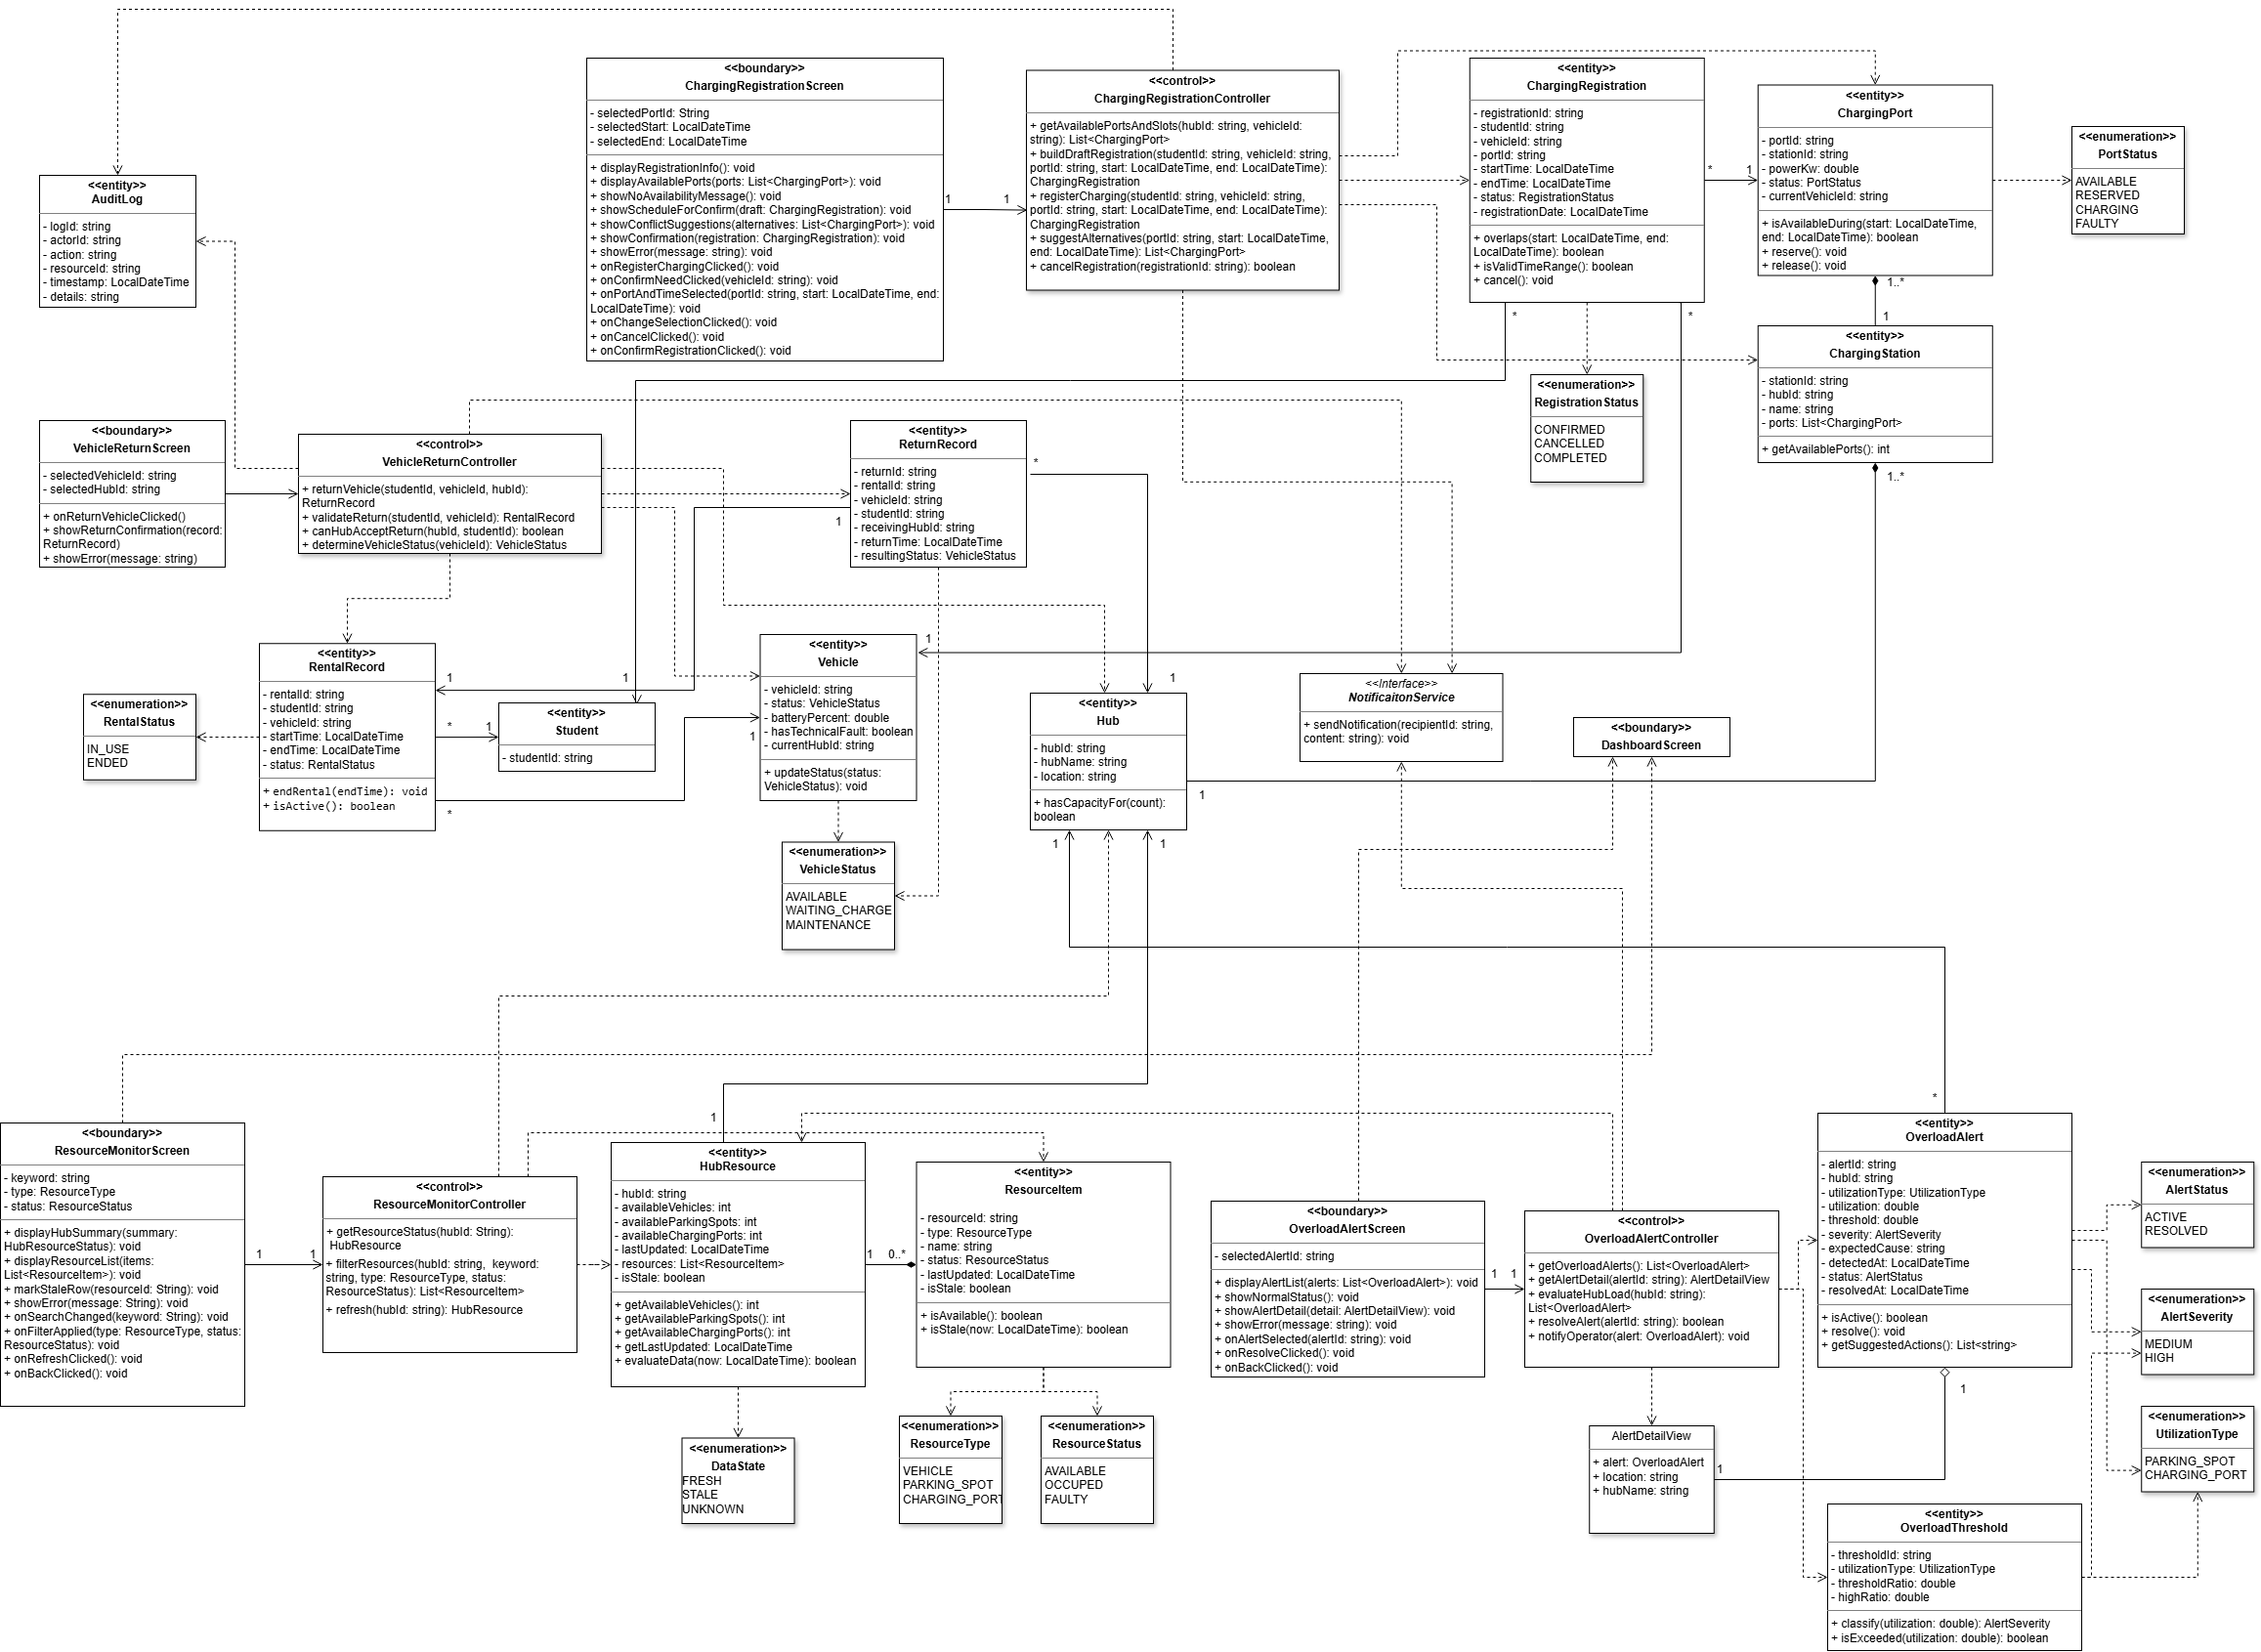
\includegraphics[width=\textwidth,height=0.82\textheight,keepaspectratio]{s3/Class_diagram_UC_6_7_9_10.png}
\end{figure}
\clearpage

\subsection{Class diagram UC11, UC12, UC16}
\begin{figure}[H]
\centering
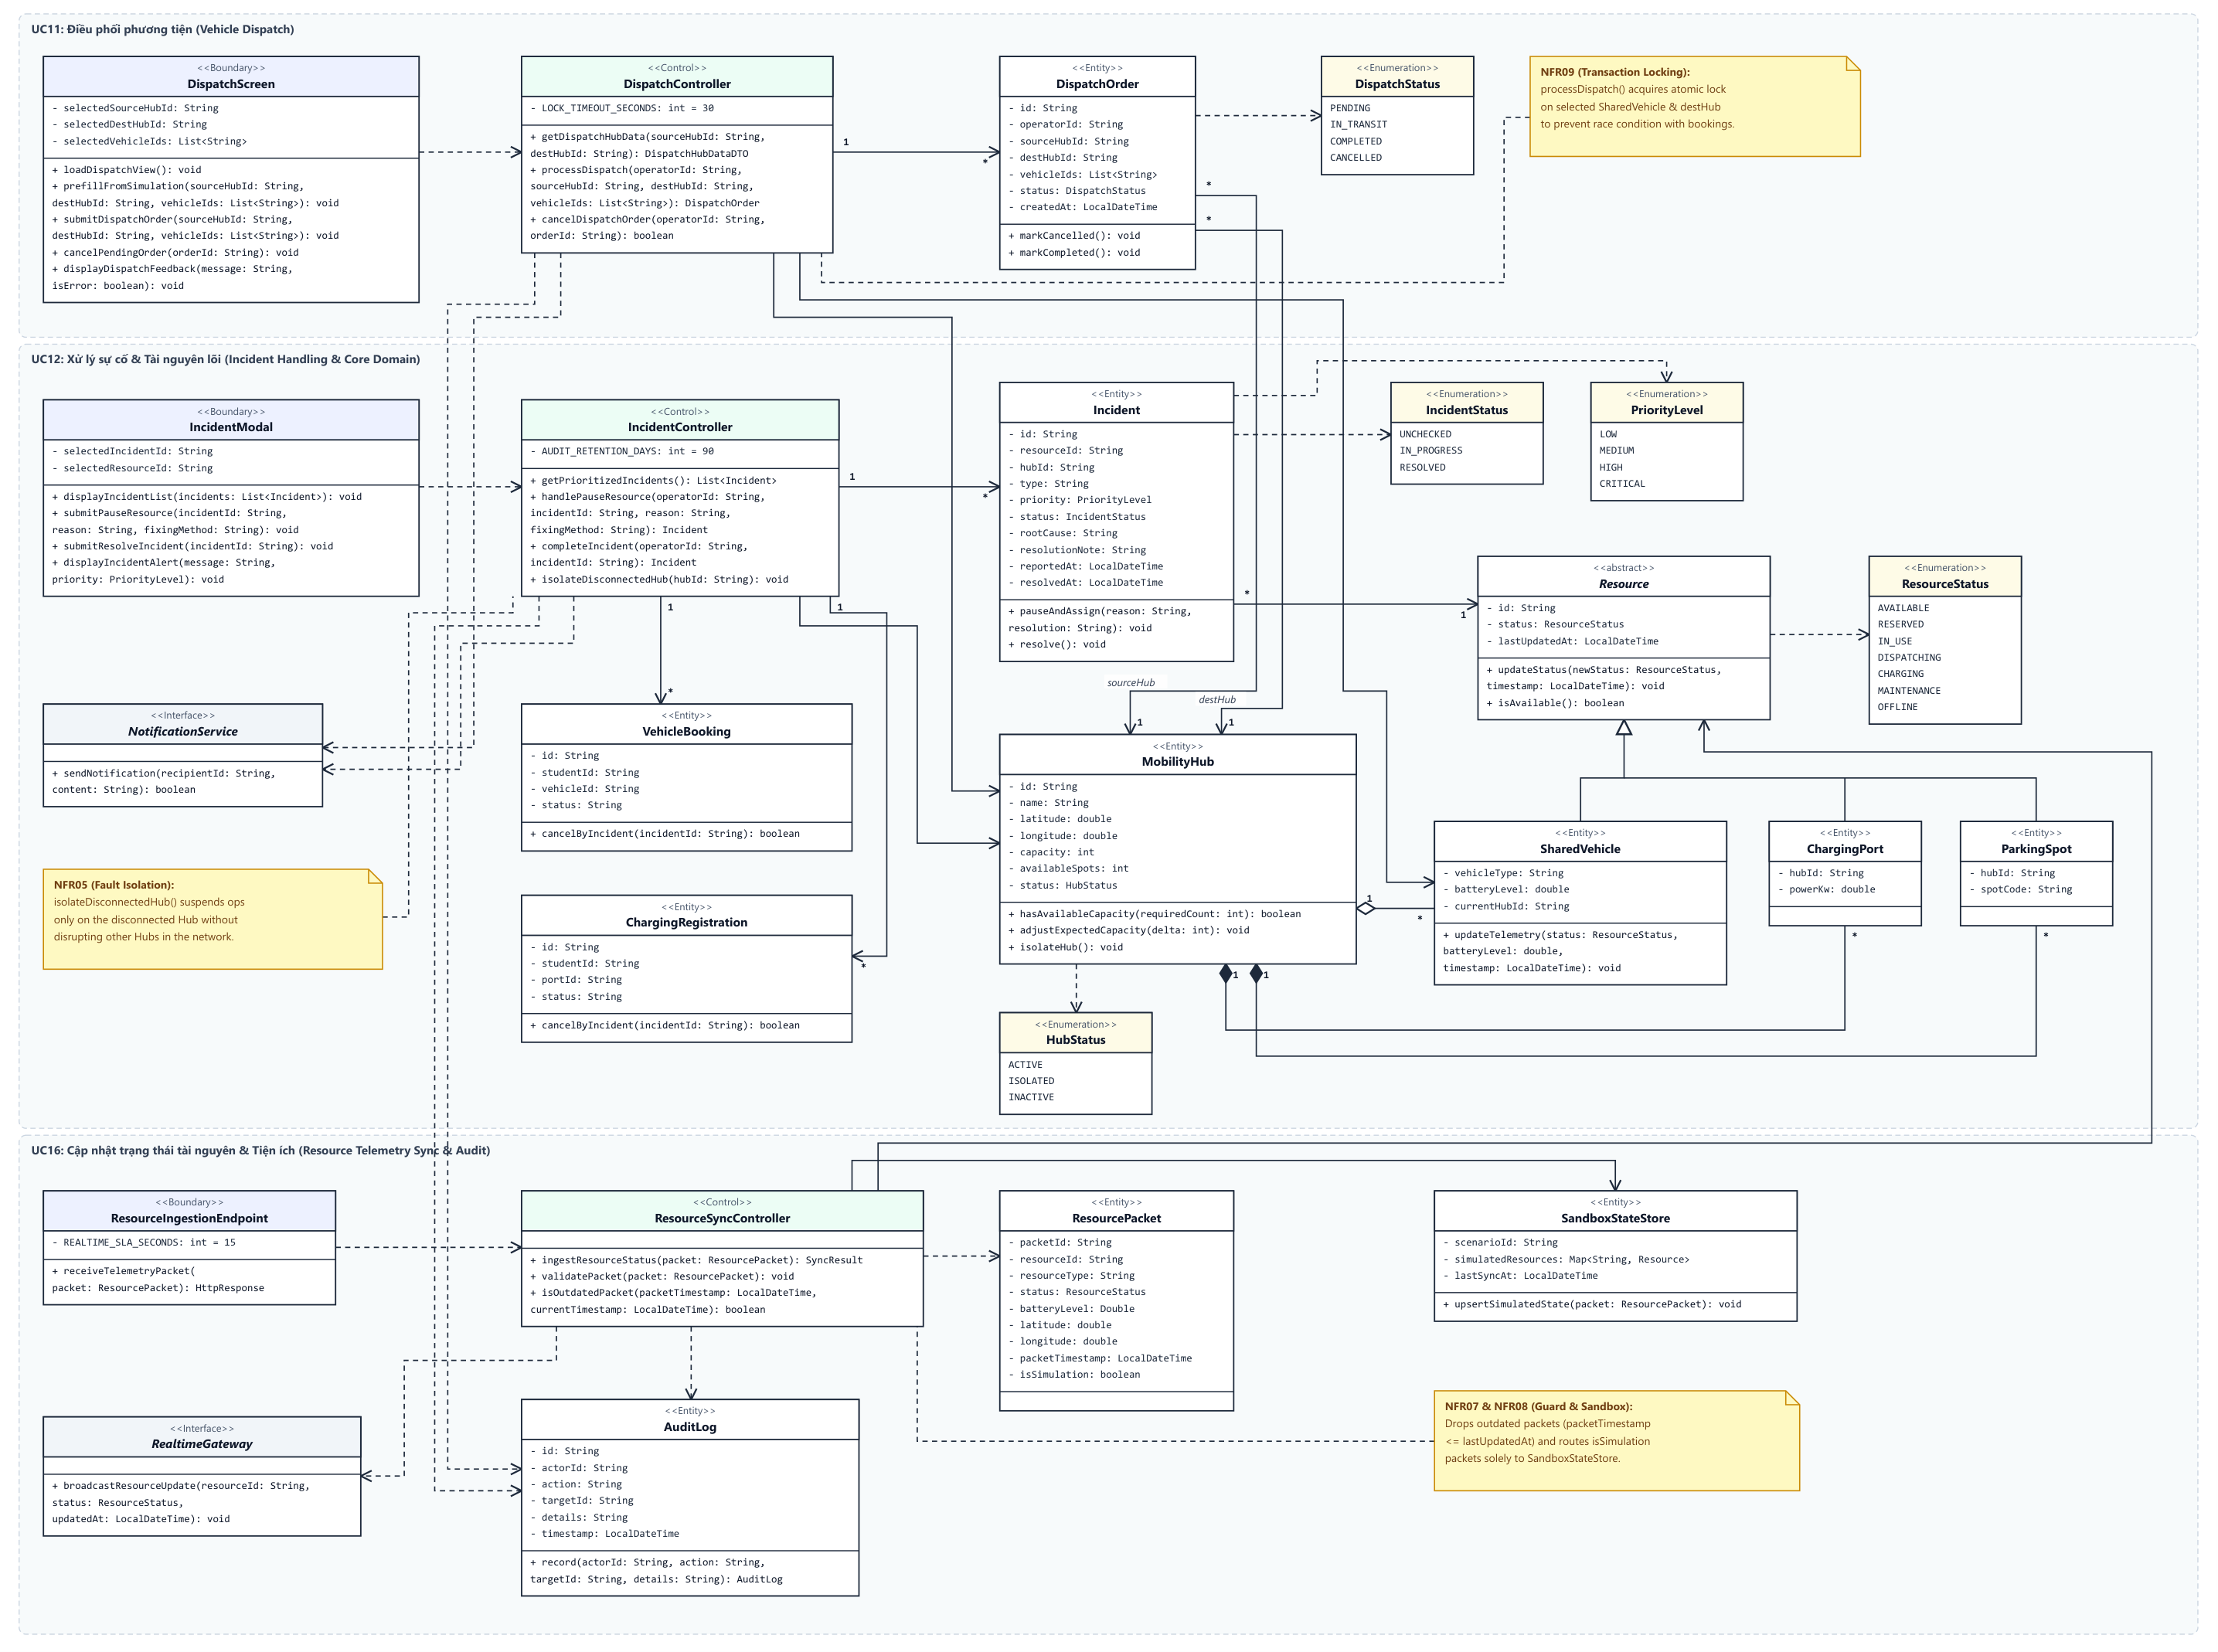
\includegraphics[width=\textwidth,height=0.82\textheight,keepaspectratio]{s3/Class_diagram_UC_11_12_16.png}
\end{figure}
\clearpage

\subsection{Class diagram UC12, UC13, UC14, UC15}
\begin{figure}[H]
\centering
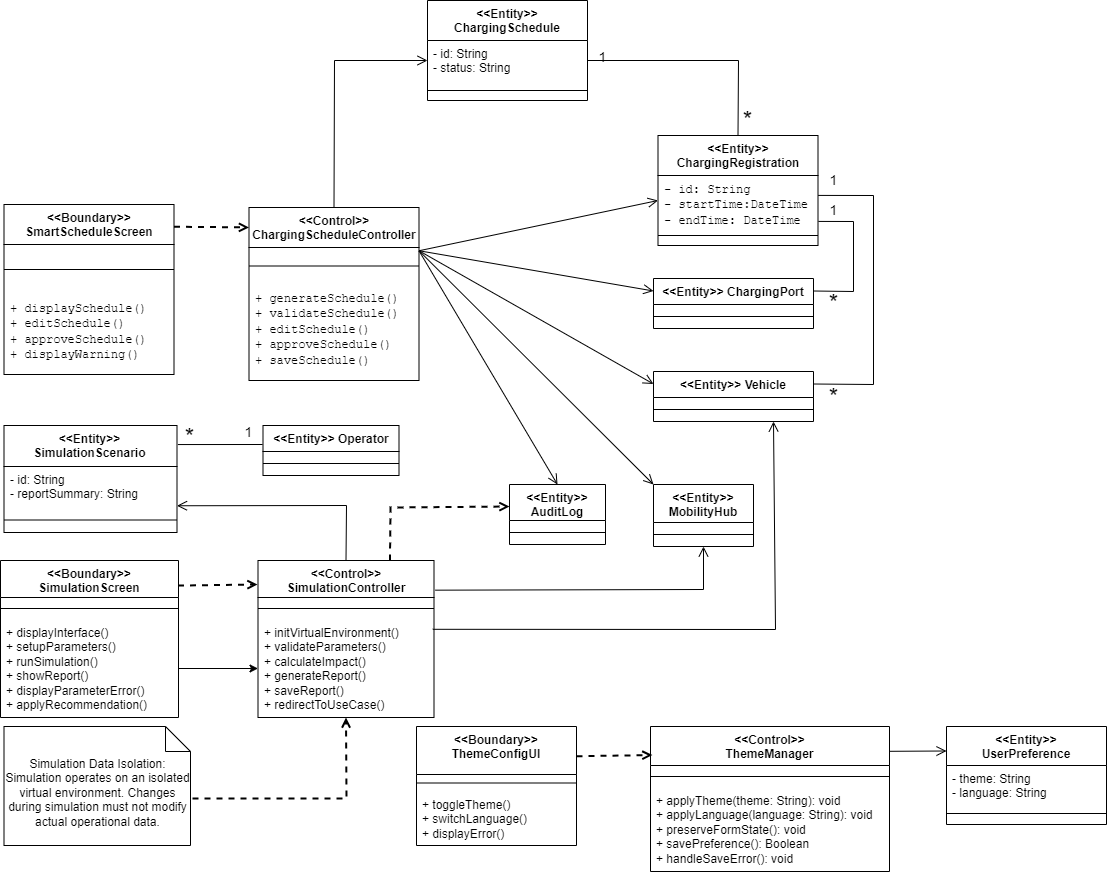
\includegraphics[width=\textwidth,height=0.82\textheight,keepaspectratio]{s3/Class_diagram_UC_13_14_15.png}
\end{figure}
\clearpage